\section{Introduction}
\label{sec:intro}

\begin{figure}[ht]
    \centering
    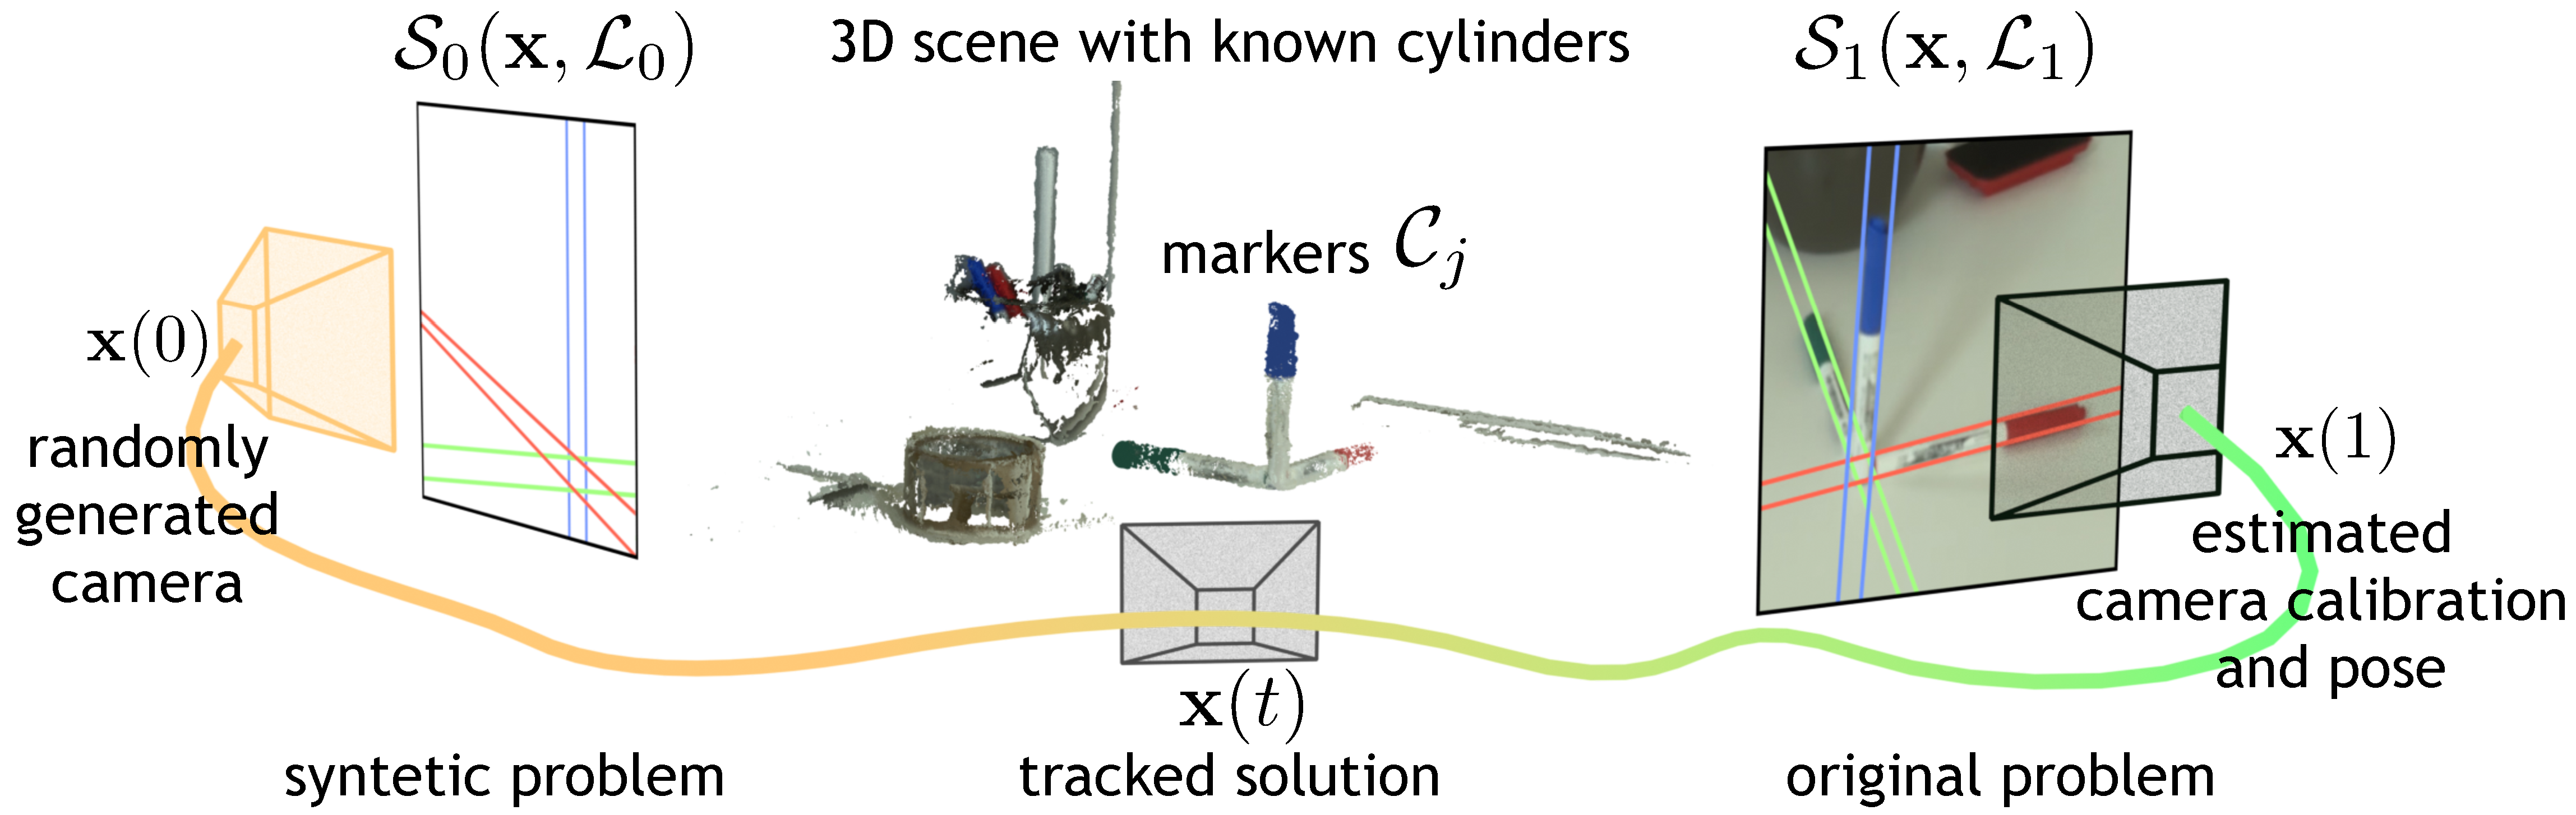
\includegraphics[width=\linewidth]{images/header_image/teaser.pdf}
    \caption{
    Our method for $N=1$  camera  and $M=3$ cylindrical objects (3 markers). The input is a known 3D scenes and images with estimated silhouette lines. The output is the calibration and the pose of the cameras that acquired the images. Rather than tackling the problem on the input data, we move to a simpler random problem with a known solution  $\mathbf{x}(0)$. Our silhouette-based parametric homotopy allows  to track $\mathbf{x}(0)$ to  the solution $\mathbf{x}(1)$  of the original problem. Our formulation support multiple cylinders and multiple images.\label{fig:homotopy}}
\end{figure}

%region Punch line
Camera calibration and camera localization are fundamental problems in Computer Vision, underpinning most, if not all, Computer Visions tasks.
%endregion

%region What is the problem
\paragraph{Camera calibration} consists in estimating the intrinsic parameters of a camera, such as focal length, principal point, and lens distortion coefficients, which are essential for accurate image formation.
Camera calibration can be split into classic camera calibration and automatic camera calibration.

Classic camera calibration typically rely on correspondences between the 3D world and the 2D image plane to estimate the camera's intrinsic parameters.
Depending on the real world object a variety of techniques can be used. Common world object choices include points, lines, planar surfaces, approximated proper quadrics.

Point based techniques often make use of fiducial markers like checkerboard patterns~\cite{Zhang2000}\ref{fig:checkerboard}, and AprilTags~\cite{\apriltag}\ref{fig:apriltags}.

Line based techniques, such as vanishing points~\cite{guo23vanishing}, can be used to estimate the camera's intrinsic parameters from the vanishing points of parallel lines in the scene.

Planar surfaces techniques, such as the one proposed by Sturm~\cite{Sturm2004}, use planar surfaces to estimate the camera's intrinsic parameters from homography between a plane and the image plane, geometric constraints like tangency, pallelism and more generally angles between planar surfaces.

Self-calibration techniques estimate the camera's intrinsic parameters directly from image data, without requiring known correspondences with the 3D world. These methods rely on geometric constraints embedded in multiple views of the scene. Classical approaches such as the Kruppa equations~\cite{Maybank1992} use correspondences between images to estimate the fundamental matrix, which constrains the image of the absolute conic (IAC), allowing recovery of the intrinsics. Extensions such as the dual absolute quadric (DAQ) approach~\cite{Triggs1997} formulate the problem in terms of projective-to-metric reconstruction, leveraging multiple uncalibrated views. Planar self-calibration methods~\cite{Pollefeys1999, Li2024} estimate homographies between images of planar surfaces to derive constraints on the camera intrinsics, with recent work addressing challenging capture geometries such as circular oblique flights. Techniques based on vanishing points~\cite{guo23vanishing} exploit structural regularities in man-made environments to constrain focal length and principal point. Special camera motions, like pure rotation~\cite{Hartley1994}, can simplify the problem by directly relating image correspondences to intrinsic parameters. Finally, bundle adjustment with self-calibration~\cite{Fitzgibbon2001} jointly refines the intrinsic parameters, camera poses, and 3D structure by minimizing reprojection errors.

Finally in recent years, machine learning techniques have been increasingly integrated into the self-calibration pipeline to address limitations of purely geometric methods, especially under challenging conditions such as low texture or ambiguous correspondences. In these hybrid approaches, deep neural networks are primarily employed for robust feature detection, correspondence estimation, depth prediction, or motion estimation, while the actual estimation of camera intrinsics remains grounded in geometric constraints. For instance, Hagemann et al.~\cite{Hagemann2023} combine learned feature extraction with a differentiable bundle adjustment framework to jointly estimate motion, structure, and intrinsics from video sequences. Similarly, Hogan et al.~\cite{Hogan2023} propose a self-supervised online system for real-time camera calibration in automotive applications, where deep learning aids pose estimation, but intrinsic parameter updates are still based on geometric models. Although fully end-to-end intrinsic estimation methods exist~\cite{Satouri2023}, most practical systems continue to leverage geometry as the core of self-calibration, with learning components improving robustness and generalization.

Exampless of aformentioned techniques can be seen in Figure~\ref{fig:calibration_examples}

\begin{figure}[b]
    \centering
    \subfloat[Checkerboard pattern]{
        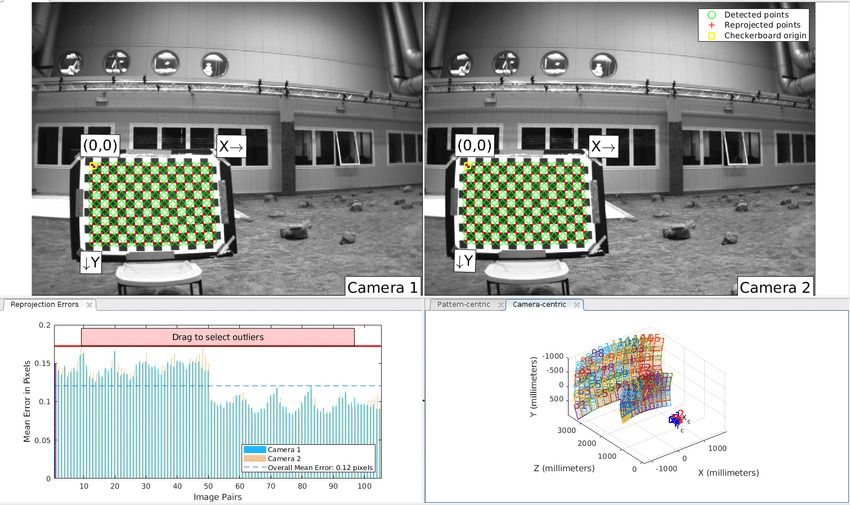
\includegraphics[width=0.23\linewidth]{images/calibration/zhang.jpg}
        \label{fig:checkerboard}
    }
    \subfloat[April tags]{
        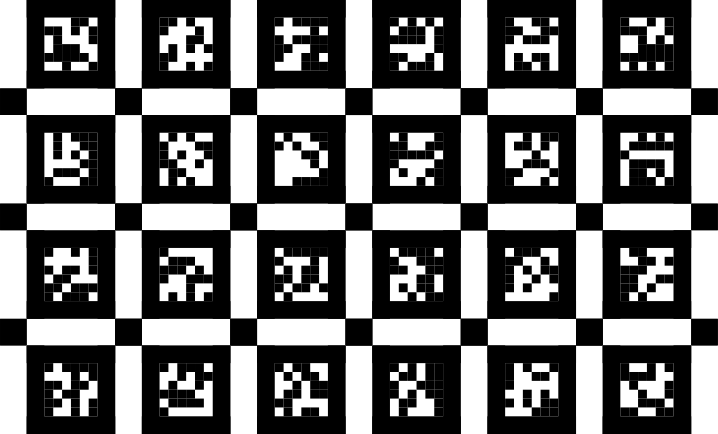
\includegraphics[width=0.23\linewidth]{images/calibration/apriltags.png}
        \label{fig:apriltags}
    }
    \subfloat[Structure from Motion]{
        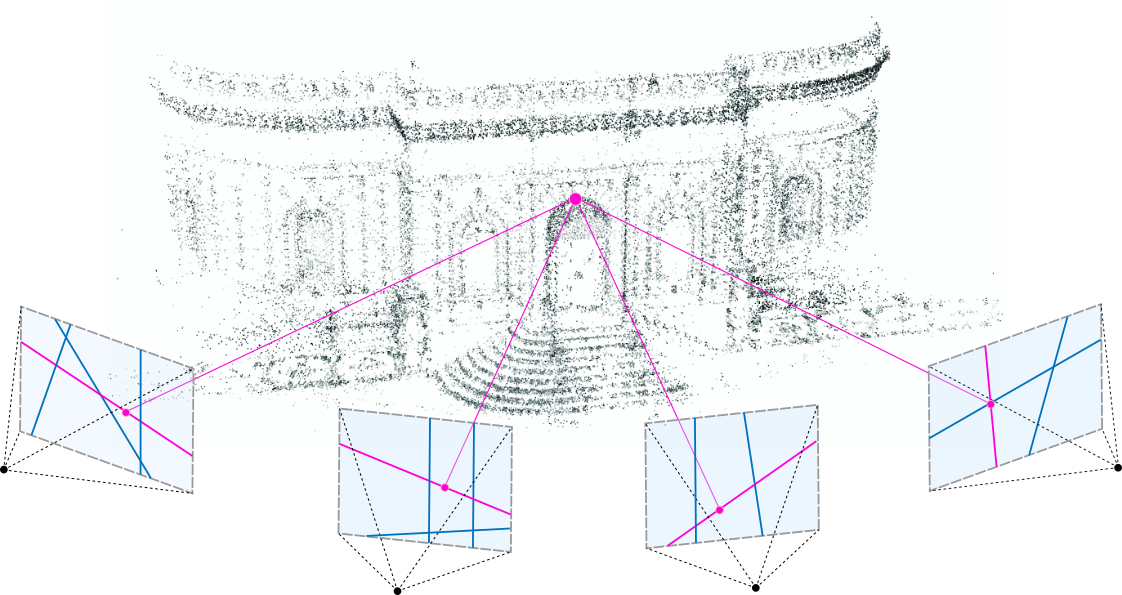
\includegraphics[width=0.23\linewidth]{images/calibration/sfm.png}
        \label{fig:sfm}
    }
    \subfloat[Surface of revolutions]{
        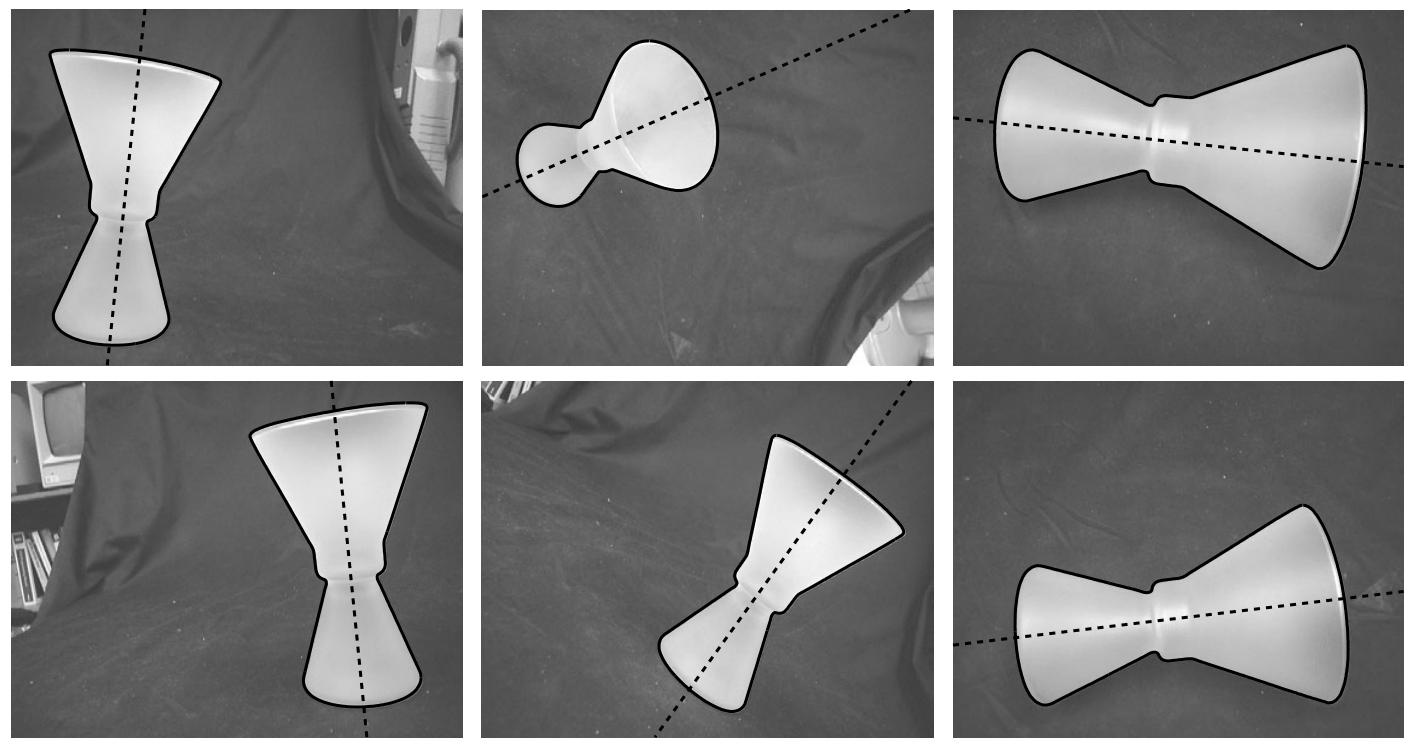
\includegraphics[width=0.23\linewidth]{images/calibration/surface_of_revolution.png}
        \label{fig:surface_of_revolutions}
    }
    \hspace{0.1\linewidth}
    \caption{Examples of various calibrations and autocalibration techniques}
    \label{fig:calibration_examples}
\end{figure}

\paragraph{Camera localization} refers to estimating the six degrees of freedom (6DoF) camera pose with respect to a pre-built 3D model or scene representation. Accurate camera localization is crucial for numerous applications such as autonomous navigation, augmented and mixed reality, or loop closure in SLAM systems. Structure-based localization methods rely on matching 2D features extracted from a query image to 3D points in the scene model, typically built using Structure-from-Motion (SfM) or SLAM pipelines. A large body of work has focused on improving the scalability~\cite{Sattler2015, Li2020}, efficiency~\cite{Sarlin2019SuperGlue, Gojcic2020}, and robustness~\cite{Sattler2018Benchmarking, Revaud2019R2D2, Dusmanu2019SuperPoint} of this matching process, particularly under challenging conditions such as viewpoint changes, lighting variations, or seasonal differences. Establishing reliable 2D-3D correspondences remains the primary bottleneck, with a well-known trade-off between descriptor invariance and discriminative power~\cite{Schonberger2016}. Recent methods combine learned local descriptors~\cite{DeTone2018SuperPoint, Sarlin2020SuperGlue} with global scene priors~\cite{Taira2018, Chen2021ACNe} or hybrid retrieval pipelines~\cite{Sattler2019Hierarchical} to reduce the dependency on exhaustive feature matching.

Multiple works explore alternative training and evaluation paradigms, including simulation-based data augmentation~\cite{Wang2022, Chen2022TransLo}, synthetic-to-real transfer~\cite{Tang2023}, or end-to-end learning of localization pipelines~\cite{Luo2020}. While purely learning-based methods show promise in generalization, geometry-based approaches remain the state-of-the-art for high-accuracy pose estimation in large-scale environments.

%end region

%region Why is it important/interesting?

A wide range of applications such 3D reconstruction, robotics, and extended reality works on top of those two building blocks.

%endregion


While point-based methods are widely used and effective, they often struggle in challenging scenarios, such as those with limited texture, occlusions, or noise. In contrast, higher-order geometric primitives, such as cylinders, offer a more robust alternative. Cylinders are prevalent in many environments and can be easily detected in images, making them suitable for calibration and localization tasks.

In this work, we focus on camera calibration \emph{and} localization from \emph{cylinders}, that are common and easily detectable structures in many man-made environments, ranging from architectural elements (\emph{e.g.}, pipes, handrails) to household objects (\emph{e.g.}, bottles, cans, furniture legs) and infrastructure components (\emph{e.g.}, street lamps, utility poles, tube lights).
While calibration and pose estimation are traditionally treated as separate problems, we build upon the geometric constraints introduced in~\cite{gummeson22pose} to develop a novel formulation that  estimates both the camera pose and the intrinsic calibration matrix. Under the assumption of constant intrinsics, this enables full camera resection directly from images of known 3D cylinders.

The core idea, illustrated in Figure~\ref{fig:homotopy}, is to leverage the known 3D geometry to simplify the estimation process. The geometric constraints between the known cylinders and the unknown camera parameters form a system of nonlinear equations $\mathcal{S}_1(\mathbf{x}, \mathcal{L}_1)$. Instead of directly solving this complex system $\mathcal{S}_1$ with traditional algebraic methods like Gröbner basis or resultants, which are prone to numerical instability and scalability issues, we take a different approach. We generate a, \emph{virtual system} $\mathcal{S}_0(\mathbf{x}, \mathcal{L}_0)$ designed around the very same 3D scene and a configuration of synthetic cameras  with random but known parameters. By design, we know the solution $\mathbf{x}(0)$ for $\mathcal{S}_0$, since it corresponds to the parameters we used to generate the synthetic cameras. Then, we continuously track the known solution $\mathbf{x}(0)$ as we transform the problem towards the original, system $\mathcal{S}_1$, using a tailored homotopy continuation parametrized in terms of silhouette lines.  At the end, we obtain the desired calibration and pose $\mathbf{x}(1)$.
By using this approach, we influence the trajectory of the solutions, guiding the solver toward more plausible configurations.
We couple our solver with dedicated initialization, and post-processing steps.
Compared to existing methods, our approach is not only more general -- being capable of  estimating both camera calibration and pose, unlike alternatives that address only one of the two task -- but also achieves superior accuracy and improved robustness to noise, as demonstrated by our experiments.

% All in all, our contributions can be summarized as follows:
% \begin{itemize}[noitemsep]
%     \item We present a \emph{unified solution} for calibration and pose estimation, unlike existing approaches that typically address these two problems separately.
%     \item We conceive a \emph{novel solver},  that, exploiting a silhouette-based parametrization,   simplifies the original problem into a one with a known solution, which is then lifted via homotopic continuation to the original one.
%     \item We introduce a \emph{dedicated initialization} step that leverages the known 3D geometry of cylinders to improve convergence and robustness.
%     \item We propose a geometric \emph{correction step} to deal with unavoidable spurious solutions.
%     \item Our method is  \emph{more accurate} and \emph{robust} to noise compared to alternative solutions.
% \end{itemize}

In this paper we will go through:
\begin{itemize}[noitemsep]
    \item Section~\ref{sec:related} reviews related work on camera calibration and pose estimation from advanced geometric primitives, in particular cylindrical objects.
    \item Section~\ref{sec:problem_formulation} gives a high detail formulation of the problem: input, outputs, and constraints.
    \item Section~\ref{sec:constraints} summarize relevant quadrics theory: dual quadrics, null space, tangency.
    \item Section~\ref{sec:homotopy} summarize relevant homotopy continuation theory.
    \item Section~\ref{sec:method} presents our homotopy-based solver for the problem.
    \item Section~\ref{sec:iterating_procedure} describe best practices on how to initialize and iterate the solver.
    \item Section~\ref{sec:postprocessing} describes our post-processing step to correct spurious solutions.
    \item Section~\ref{sec:experiments} evaluates our method on synthetic and real-world datasets, demonstrating its effectiveness and robustness.
    \item Section~\ref{sec:conclusions} concludes the paper and discusses future work.
    \item Appendix~\ref{sec:appendix} provides additional details on the implementation of the different algorithms.
\end{itemize}

%Since homotopy solvers could not directly enforce inequality constraints, it may happen that during the tracking of the solutions some retrieved parameters violates physical constraints. Thus we  Our post-processing step identifies and corrects spurious solutions, improving the physical validity of the final camera parameters. 

%While the computational time of the solution is not suited to be used as a validation method for a RANSAC approach, the method is well suited to find models to then validate through RANSAC.
%\lm{Qui diciamo velocemente come è la struttura del paper}\eb{Com'è?}
%The paper is structred as follow: after laiding down the problem formulation (Section \todo{XX}) and reviewing s the multi-view-geometry of cylinders (Section \todo{XX}), we present our homotopy based solver  (Section \todo{XX})  coupled with our post-processing step (Section \todo{XX}). The benefits of our apporach are then evaluated in Section \todo{XX}.
%In this paper, we extend this line of research by addressing the more challenging scenario where the camera is not assumed to be calibrated. We introduce a novel approach for jointly estimating camera intrinsics and pose from multiple views of known cylindrical objects. Our method is enabled by a new solver based on homotopy continuation, which handles the non-linear constraints arising from the projection of cylindrical silhouettes.

%A key challenge in this formulation lies in the presence of spurious solutions—combinations of intrinsic parameters and rotations that satisfy the projection equations but do not correspond to physically valid configurations. Because standard homotopy continuation methods cannot enforce inequality constraints (such as positive focal lengths), we propose a novel post-processing step that filters out ambiguous solutions algebraically, ensuring geometric validity without artificial regularization.

%This results in a complete and practical framework for camera calibration and localization using a minimal, easy-to-setup set of cylindrical objects. We validate our approach on both synthetic and real-world datasets, demonstrating accurate and robust performance even in challenging conditions.